\documentclass[conference]{IEEEtran}
\IEEEoverridecommandlockouts
% The preceding line is only needed to identify funding in the first footnote. If that is unneeded, please comment it out.
\usepackage{cite}
\usepackage{amsmath,amssymb,amsfonts}
\usepackage{algorithmic}
\usepackage{graphicx}
\usepackage{textcomp}
\usepackage{xcolor}

\usepackage[acronym]{glossaries}
\usepackage{tikz}
\usetikzlibrary{positioning, shadows, fit}
\usepackage{float}
\usepackage{booktabs}
\usepackage{url}

% Acronyms  
\newacronym{ai}{AI}{artificial intelligence}
\newacronym{ml}{ML}{machine learning}
\newacronym{automl}{AutoML}{automated machine learning}
\newacronym{hcai}{HCAI}{human-centered artificial intelligence}
\newacronym{hgml}{HGML}{human-guided machine learning}
\newacronym{gui}{GUI}{Graphical User Interface}
\newacronym{ui}{UI}{User Interface}
\newacronym{dl}{DL}{Deep Learning}
\newacronym{hci}{HCI}{Human-Computer Interaction}  
\newacronym{auc_roc}{AUC-ROC}{Area Under the Receiver Operating Characteristic Curve}  
\newacronym{mae}{MAE}{Mean Absolute Error}  
\newacronym{rmse}{RMSE}{Root Mean Squared Error}  
\newacronym{shap}{SHAP}{SHapley Additive exPlanations}  
\newacronym{lime}{LIME}{Local Interpretable Model-agnostic Explanations}  
\newacronym{xai}{XAI}{Explainable Artificial Intelligence}
\newacronym{crp}{CRP}{clinical research professional}
\newacronym{hamelin}{HAMELIN}{Human-guided Automated Machine Learning for Clinical Studies}
\newacronym{icu}{ICU}{intensive care unit}
\newacronym{llm}{LLM}{large language model}


\def\BibTeX{{\rm B\kern-.05em{\sc i\kern-.025em b}\kern-.08em
    T\kern-.1667em\lower.7ex\hbox{E}\kern-.125emX}}
\begin{document}

\title{Towards a Human-Guided AutoML Application for Democratizing Predictive Modeling in Clinical Research\\
\thanks{This work has been supported by grant  PID2023-146243OB-I00 funded by MICIU/AEI/10.13039/501100011033 and by ``ERDF/EU''.}
}

\author{\IEEEauthorblockN{1\textsuperscript{st} Diego Garc\'ia-Prieto}
\IEEEauthorblockA{\textit{Dept. of Mathematics, Statistics and Computer Science} \\
\textit{University of Cantabria}\\
Santander, Spain \\
diego.garciaprieto@unican.es}
\and
\IEEEauthorblockN{2\textsuperscript{nd} Camilo Palazuelos}
\IEEEauthorblockA{\textit{Dept. of Mathematics, Statistics and Computer Science} \\
\textit{University of Cantabria}\\
Santander, Spain \\
camilo.palazuelos@unican.es}
\and
\IEEEauthorblockN{3\textsuperscript{rd} Rafael Duque}
\IEEEauthorblockA{\textit{Dept. of Mathematics, Statistics and Computer Science} \\
\textit{University of Cantabria}\\
Santander, Spain \\
rafael.duque@unican.es}
\and
\IEEEauthorblockN{4\textsuperscript{th} Luc\'ia Lav\'in-Alconero}
\IEEEauthorblockA{\textit{Clinical Trials Agency Valdecilla-IDIVAL} \\
\textit{Marqu\'es de Valdecilla University Hospital}\\
Santander, Spain \\
lucia.lavin@idival.org}
}

\maketitle

\begin{abstract}
Clinical research faces a significant gap between advanced machine learning capabilities and their practical adoption by non-technical researchers. Existing AutoML tools treat clinical data as generic datasets, ignoring the methodological particularities of patient registries, observational studies and clinical trials. To address this, we present HAMELIN, an AutoML application under active development that bridges this gap through a protocol-aware interface aligned with Human-Guided Machine Learning principles. HAMELIN enables clinical researchers to build predictive models without coding, incorporating their domain knowledge to guide the process.
\end{abstract}

\begin{IEEEkeywords}
machine learning for healthcare, automated machine learning, human-guided machine learning, clinical research, protocol-aware systems
\end{IEEEkeywords}

\section{Introduction}
\label{sec:introduction}

The rapid integration of \gls{ai} into medicine faces a key challenge: clinicians have domain knowledge and research hypotheses but lack technical skills for complex \gls{ml} pipelines, while data scientists can build advanced models but often lack the clinical context to ensure validity and relevance \cite{gisselbaek2025bridging}. This expertise gap hinders the adoption of \gls{ai} in clinical research.

Current state-of-the-art \gls{automl} platforms fail to bridge this gap for clinical researchers \cite{waring2020automated}. They treat datasets as generic matrices, ignoring structures inherent to clinical research, such as patient registries, observational studies, and clinical trials. They are not protocol-aware, making it difficult to distinguish between variables that define study populations (inclusion criteria) and those measuring outcomes (endpoints). Moreover, their black-box nature complicates interpretation and poorly adapts to clinical particularities, such as temporal data organization or semantic distinctions between efficacy and safety variables.  
Incorporating domain knowledge into the modeling process is essential \cite{sirocchi2024medical}. \gls{hamelin}, based on \gls{hgml} principles, provides a no-code, protocol-aware environment where clinicians and data scientists collaborate using a shared language. By explicitly defining variables, distinguishing endpoints from exposures, and interventions from covariates, \gls{hamelin} facilitates the development of predictive models that are clinically coherent and aligned with the structural requirements of research designs, effectively bridging the gap between technical expertise and clinical relevance.

\section{Background}
\label{sec:background}

\subsection{Clinical Research Methodologies}
\label{subsec:clinical_research}

Clinical research employs distinct frameworks, each with specific design principles and analytical constraints \cite{kahlert2017control}. Patient registries collect real-world, long-term data from people who share the same medical condition. Observational studies test specific hypotheses about exposure-outcome associations without intervention, requiring adjustment for confounding variables. Clinical trials evaluate interventions through randomization, blinding and rigorous protocols defining inclusion/exclusion criteria, temporal phases (screening, intervention, follow-up) and endpoint hierarchies (primary for efficacy, secondary for safety).

These distinctions impose specific requirements on predictive modeling that generic \gls{ml} pipelines ignore \cite{gao2025confounder}. A model trained without awareness of these constraints risks producing invalid results.

\subsection{Related Work}
\label{subsec:related_work}

\gls{automl} tools such as Auto-sklearn \cite{autosklearn}, AutoGluon \cite{autogluon}, H2O \cite{h2o3}, and Ludwig \cite{ludwig} have successfully automated the \gls{ml} pipeline \cite{he2021automl}, but remain largely domain-agnostic. They cannot distinguish variable hierarchy (primary endpoints vs. secondary endpoints vs. exposures), handle complex inclusion/exclusion logic, or recognize temporal data disposition across protocol phases. No tool to date adapts to the distinct requirements of patient registries, observational studies and clinical trials within a unified interface. This is precisely the gap addressed by protocol-aware \gls{ai} systems \cite{zainleveraging}.

\gls{hgml} \cite{gil2019towards} is an approach in which domain experts guide and influence the learning process, rather than relying solely on automated algorithms. It promotes collaborative workflows where experts validate intermediate decisions and shape model behaviour.

\subsection{Ludwig AutoML}
\label{subsec:ludwig}

 Ludwig \cite{ludwig} is an \gls{automl} tool which automates the full \gls{ml} workflow, including end-to-end model training, algorithm selection based on data characteristics, performance evaluation with multiple metrics and validation schemes, hyperparameter optimisation and seamless inference on new data. Being YAML-based, a human-readable data-serialization format, it allows pipelines to be specified declaratively without programming. The choice of Ludwig as an backend is motivated by its ease of configuration, strong community support and active open-source development, which ensure long-term maintainability \cite{palazuelos2024non}.


\section{Application}
\label{sec:application}

\gls{hamelin} is an application designed to operationalize \gls{hgml} principles for clinical research. The system design was guided by mockups based on real clinical research protocols provided by clinical research professionals. This ensures that the interface terminology, workflow structure, and validation mechanisms align with actual clinical research practices.

\subsection{Architecture}

The system architecture, illustrated in Figure~\ref{fig:system_architecture}, follows a three-layer modular design. The interface layer provides a graphical environment for dataset loading, configuration, and visualization. The core logic layer connects the interface to the \gls{automl} engine, handling validation, command translation, and configuration generation. The \gls{automl} layer utilizes Ludwig (v0.10.4) to perform automated training, algorithm selection, and hyperparameter optimization.

\begin{figure}[H]
\centering
\scalebox{0.75}{
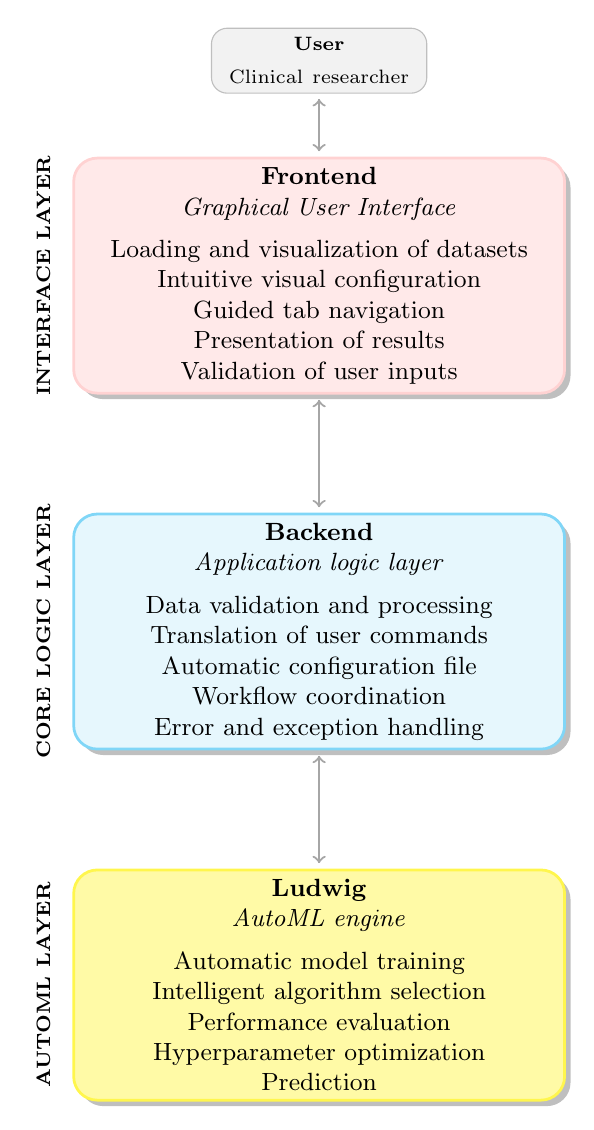
\begin{tikzpicture}[
    node distance=1.5cm, % separación vertical entre nodos
    box/.style={
        rectangle,
        draw,
        text width=6cm,
        text centered,
        minimum height=2cm,
        rounded corners=0.3cm,
        drop shadow,
        line width=1pt,
        font=\small
    },
    frontend/.style={box, fill=pink!35, draw=pink!70},
    backend/.style={box, fill=cyan!10, draw=cyan!50},
    ludwig/.style={box, fill=yellow!35, draw=yellow!70},
    arrow/.style={->, thick, color=gray!70, line width=0.8pt, shorten >=2pt, shorten <=2pt},
]

% Nodos principales (vertical)
\node[frontend] (frontend) at (0,0) {
    \textbf{Frontend}\\
    \textit{Graphical User Interface}\\[1.5mm]
    Loading and visualization of datasets\\
    Intuitive visual configuration\\
    Guided tab navigation\\
    Presentation of results\\
    Validation of user inputs
};

\node[backend, below=1.5cm of frontend.south, anchor=north] (backend) {
    \textbf{Backend}\\
    \textit{Application logic layer}\\[1.5mm]
    Data validation and processing\\
    Translation of user commands\\
    Automatic configuration file\\
    Workflow coordination\\
    Error and exception handling
};

\node[ludwig, below=1.5cm of backend.south, anchor=north] (ludwig) {
    \textbf{Ludwig}\\
    \textit{AutoML engine}\\[1.5mm]
    Automatic model training\\
    Intelligent algorithm selection\\
    Performance evaluation\\
    Hyperparameter optimization\\
    Prediction
};

% Flechas bidireccionales verticales
\draw[arrow] (frontend.south) -- (backend.north);
\draw[arrow] (backend.north) -- (frontend.south);
\draw[arrow] (backend.south) -- (ludwig.north);
\draw[arrow] (ludwig.north) -- (backend.south);

% Usuario
\node[above=0.8cm of frontend.north, 
      rectangle, 
      draw=gray!50, 
      fill=gray!10, 
      text width=2.5cm, 
      text centered,
      rounded corners=0.2cm] (user) {
    \scriptsize \textbf{User}\\
    \scriptsize Clinical researcher
};
\draw[arrow] (user.south) -- (frontend.north);
\draw[arrow] (frontend.north) -- (user.south);

% Etiquetas de capas rotadas 90 grados, alineadas con el centro vertical de cada nodo
\node[anchor=center, rotate=90] at ([xshift=-3.5cm]frontend.center) {\scriptsize \textbf{INTERFACE LAYER}};
\node[anchor=center, rotate=90] at ([xshift=-3.5cm]backend.center) {\scriptsize \textbf{CORE LOGIC LAYER}};
\node[anchor=center, rotate=90] at ([xshift=-3.5cm]ludwig.center) {\scriptsize \textbf{AUTOML LAYER}};

\end{tikzpicture}
}
\caption{System architecture}
\label{fig:system_architecture}
\end{figure}



\subsection{User Interface and Workflow}

The interface employs a tabbed navigation system that guides users through the entire \gls{ml} pipeline. This design provides clear waypoints while maintaining the analytical context, with each tab representing a distinct phase that follows the logical progression typically found in clinical research protocols (Figure~\ref{fig:workflow}). Earlier steps can be revisited if needed.

\begin{figure}[htbp]
\centering
\scalebox{0.70}{
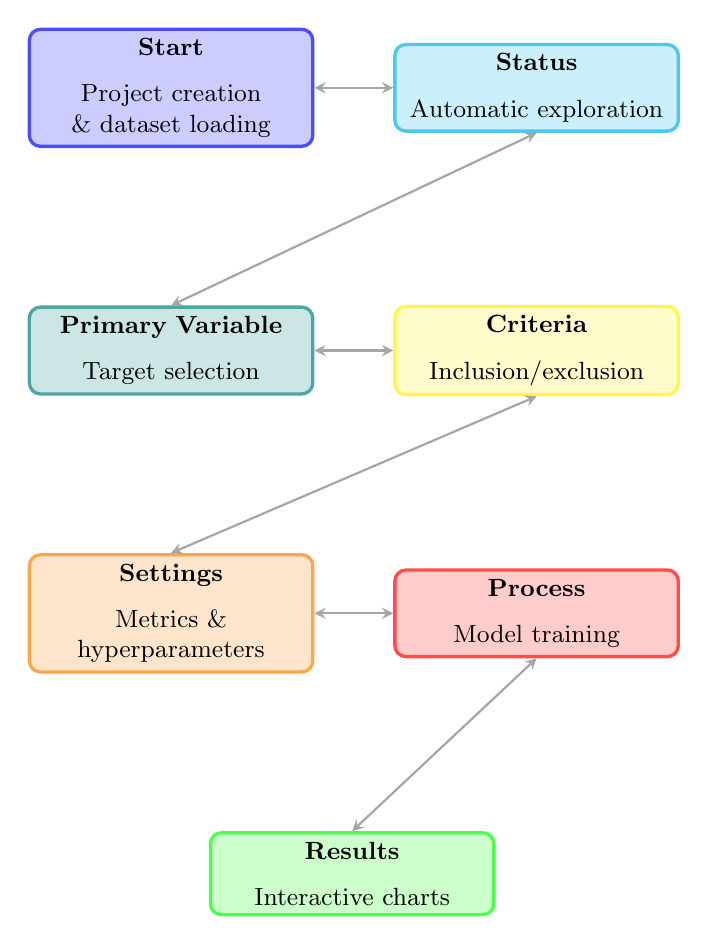
\begin{tikzpicture}[node distance=2.5cm, auto]

    % Styles
    \tikzset{
        mystep/.style={
            rectangle, rounded corners,
            minimum width=3.6cm, minimum height=1cm,
            text centered, font=\small,
            text width=3.3cm, align=center,
            line width=1.2pt
        },
        arrow/.style={thick,<->,>=stealth, gray!70}
    }

    % ---------- ROW 1 ----------
    \node (start)  [mystep, fill=blue!20, draw=blue!70]   
        {\textbf{Start}\\[2mm] Project creation \& dataset loading};

    \node (status) [mystep, fill=cyan!20, draw=cyan!70, right=1.0cm of start] 
        {\textbf{Status}\\[2mm] Automatic exploration};

    % ---------- ROW 2 ----------
    \node (primary)[mystep, fill=teal!20, draw=teal!70, below=2cm of start] 
        {\textbf{Primary Variable}\\[2mm] Target selection};

    \node (criteria) [mystep, fill=yellow!20, draw=yellow!70, right=1.0cm of primary] 
        {\textbf{Criteria}\\[2mm] Inclusion/exclusion};

    % ---------- ROW 3 ----------
    \node (settings) [mystep, fill=orange!20, draw=orange!70, below=2cm of primary] 
        {\textbf{Settings}\\[2mm] Metrics \&\\ hyperparameters};

    \node (process)  [mystep, fill=red!20, draw=red!70, right=1.0cm of settings] 
        {\textbf{Process}\\[2mm] Model training};

    % ---------- ROW 4 ----------
    \node (results)  [mystep, fill=green!20, draw=green!70, below=2cm of settings, xshift=2.3cm] 
        {\textbf{Results}\\[2mm] Interactive charts};

    % ---------- ARROWS ----------
    \draw [arrow] (start) -- (status);
    \draw [arrow] (status.south) -- (primary.north);

    \draw [arrow] (primary) -- (criteria);
    \draw [arrow] (criteria.south) -- (settings.north);

    \draw [arrow] (settings) -- (process);
    \draw [arrow] (process.south) -- (results.north);

\end{tikzpicture}
}
\caption{Clinical machine learning workflow.}
\label{fig:workflow}
\end{figure}

The workflow itself comprises seven steps: starting with project creation and dataset loading, followed by automatic dataset exploration for descriptive statistics, missing value analysis, and outcome variable identification. Users then select the target variable, with automatic detection of whether the task is classification or regression. Inclusion and exclusion criteria are defined through an intuitive interface, after which evaluation metrics, missing data strategies, and hyperparameter settings are configured. Model training is executed with real-time progress monitoring, and results are presented in a written way and through charts and confusion matrices (Figure~\ref{fig:tab-based_interface}).


\begin{figure}[ht]
    \centering
    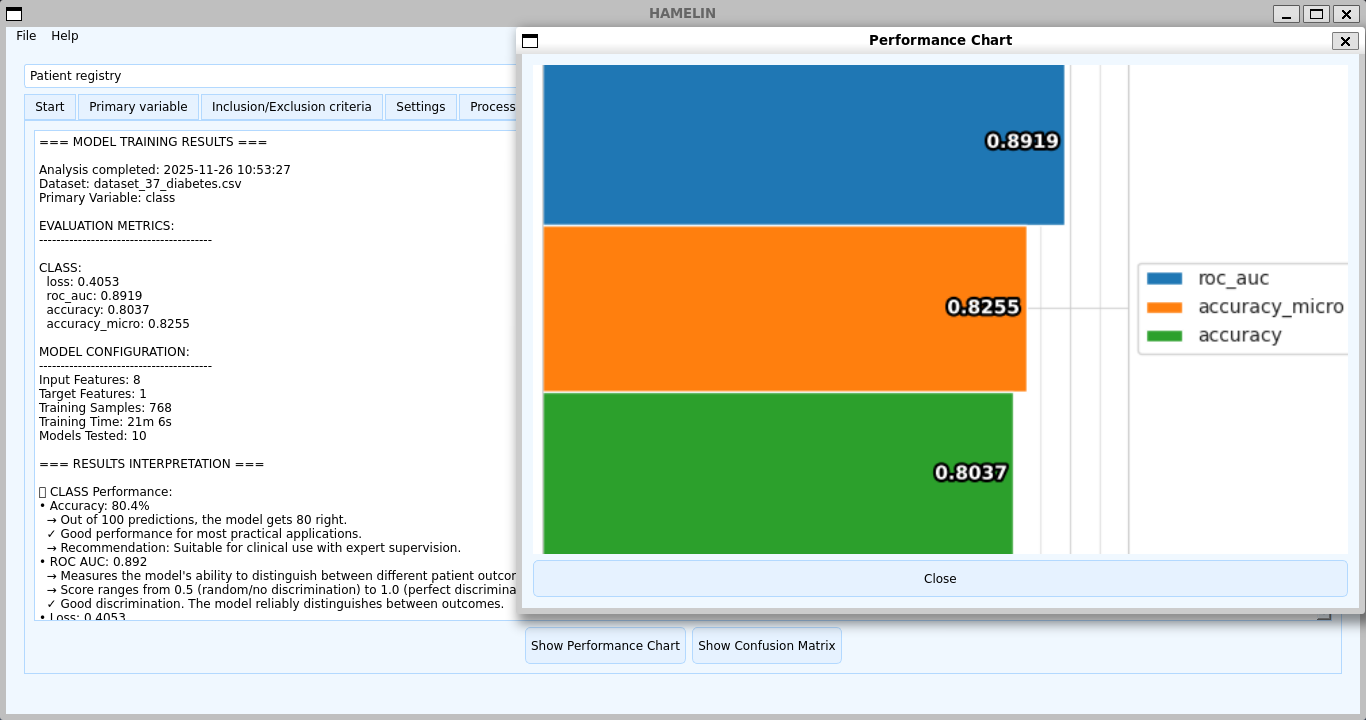
\includegraphics[width=\columnwidth]{img/Captura de pantalla 2025-11-26 111307.png}
    \caption{Training outcomes and model performance.}
    \label{fig:tab-based_interface}
\end{figure}


\section{Alignment with Human-Guided ML}
\label{subsec:hgml_alignment}

To evaluate \gls{hamelin}, we follow the \gls{hgml} criteria, which provide a structured framework to assess how domain experts can guide data use, model development, and result interpretation in interactive ML systems. Applying these criteria highlights both the strengths and limitations of \gls{hamelin} in supporting clinical researchers (Table \ref{tab:hgml_alignment}).

\begin{table}[t]
\caption{Mapping between \gls{hgml} tasks \cite{gil2019towards} and \gls{hamelin} clinical functionalities.}
\label{tab:hgml_alignment}
\centering
\scriptsize
\renewcommand{\arraystretch}{1.2}
\begin{tabular}{@{}l l@{}}
\toprule
\textbf{HGML task} & \textbf{Where in HAMELIN} \\
\midrule
\multicolumn{2}{l}{\textbf{Data Use}} \\
\midrule
\parbox[t]{0.45\columnwidth}{[VS1] Variable selection (prioritise variables)} & \parbox[t]{0.55\columnwidth}{\emph{Primary Variable}, \emph{Settings}} \\
\parbox[t]{0.45\columnwidth}{[VS2] Create new variables from existing ones} & \parbox[t]{0.55\columnwidth}{-- (external preprocessing)} \\
\parbox[t]{0.45\columnwidth}{[VS3] Change temporal / spatial framing of variables} & \parbox[t]{0.55\columnwidth}{\emph{Criteria}; protocol phases} \\
\parbox[t]{0.45\columnwidth}{[VS4] Impute missing values using other variables} & \parbox[t]{0.55\columnwidth}{\emph{Settings}} \\
\parbox[t]{0.45\columnwidth}{[VS5] Augment data using new sources} & \parbox[t]{0.55\columnwidth}{--} \\
\parbox[t]{0.45\columnwidth}{[VR1] Require inclusion / exclusion of variables} & \parbox[t]{0.55\columnwidth}{\emph{Criteria}} \\
\parbox[t]{0.45\columnwidth}{[IS1] Select instances to label / annotate} & \parbox[t]{0.55\columnwidth}{--} \\
\parbox[t]{0.45\columnwidth}{[IS2] Select subpopulation of instances} & \parbox[t]{0.55\columnwidth}{\emph{Criteria}} \\
\parbox[t]{0.45\columnwidth}{[IS3] Remove specific instances} & \parbox[t]{0.55\columnwidth}{\emph{Criteria}} \\
\parbox[t]{0.45\columnwidth}{[IS4] Define train/test split and cross-validation} & \parbox[t]{0.55\columnwidth}{\emph{Settings}} \\
\midrule
\multicolumn{2}{l}{\textbf{Model Development}} \\
\midrule
\parbox[t]{0.45\columnwidth}{[MS1] Request a specific type of model} & \parbox[t]{0.55\columnwidth}{\emph{AutoML Layer} (Ludwig)} \\
\parbox[t]{0.45\columnwidth}{[MS2] Replace the model in a prior solution} & \parbox[t]{0.55\columnwidth}{--} \\
\parbox[t]{0.45\columnwidth}{[PT1] Request specific parameter values} & \parbox[t]{0.55\columnwidth}{\emph{Settings}, Ludwig HP search} \\
\parbox[t]{0.45\columnwidth}{[SD1] Request specific data-preparation steps} & \parbox[t]{0.55\columnwidth}{\emph{Settings}} \\
\parbox[t]{0.45\columnwidth}{[SD2] Replace a data-preparation step} & \parbox[t]{0.55\columnwidth}{\emph{Settings}} \\
\midrule
\multicolumn{2}{l}{\textbf{Model Interpretation and Comparison}} \\
\midrule
\parbox[t]{0.45\columnwidth}{[QC1] Request quantities of interest / metrics} & \parbox[t]{0.55\columnwidth}{\emph{Results}} \\
\parbox[t]{0.45\columnwidth}{[QC2] Request intermediate results} & \parbox[t]{0.55\columnwidth}{--} \\
\parbox[t]{0.45\columnwidth}{[MC1] Compare solutions with different model types} & \parbox[t]{0.55\columnwidth}{--} \\
\parbox[t]{0.45\columnwidth}{[MC2] Compare solutions on different subsets of instances} & \parbox[t]{0.55\columnwidth}{--} \\
\parbox[t]{0.45\columnwidth}{[MC3] Compare solutions with same model but different data prep} & \parbox[t]{0.55\columnwidth}{--} \\
\parbox[t]{0.45\columnwidth}{[MC4] Compare solutions with same model but different parameters} & \parbox[t]{0.55\columnwidth}{--} \\
\parbox[t]{0.45\columnwidth}{[MC5] Compare two models with all other steps equal} & \parbox[t]{0.55\columnwidth}{--} \\
\parbox[t]{0.45\columnwidth}{[PC1] Several solutions with same model and varying parameter ranges} & \parbox[t]{0.55\columnwidth}{--} \\
\bottomrule
\end{tabular}
\end{table}


\gls{hamelin} offers strong support for data-centric tasks: clinicians can select variables, define inclusion/exclusion rules, and create protocol-consistent subpopulations. Temporal framing of study phases and basic missing-value handling are partially supported, but interactive data augmentation, active labeling, and fine-grained train/test split control are unsupported.

Regarding model development, \gls{hamelin} relies on the underlying \gls{automl} backend for model-family selection and hyperparameter tuning, giving users high-level control over preprocessing and training options but not detailed model choices or step-wise comparisons. In model interpretation, domain-relevant metrics are fully available, though intermediate artefacts and systematic comparisons across models or preprocessing variants are lacking. Overall, \gls{hamelin} empowers clinicians in data-centric decisions, while model-centric flexibility and advanced comparison features need further development.



\section{Conclusions}
\label{sec:conclusions}

This work presents a tool that partially satisfies the criteria for \gls{hgml}, addressing the critical gap between advanced \gls{ml} capabilities and their practical adoption in clinical research. By embedding protocol-aware constraints, the system ensures that predictive models respect temporal structures, endpoint hierarchies, and inclusion/exclusion criteria across patient registries, observational studies, and clinical trials. This design enhances clinical validity and coherence, distinguishing the approach from existing domain-agnostic \gls{automl} platforms that treat clinical datasets as generic matrices.

The evaluation indicates strong support for data-centric operations, including variable selection, subpopulation definition, and inclusion/exclusion logic. Nevertheless, model-centric tasks, such as explicit model family selection, hyperparameter specification, and systematic comparison of alternative solutions, remain partially constrained. Ongoing development aims to extend interactive control over these stages, incorporate advanced feature engineering, provenance tracking, and multi-source data integration, moving the system toward full \gls{hgml} where domain expertise can guide all aspects of the modeling process.


\begin{footnotesize}

\bibliographystyle{unsrt}
\bibliography{bibliography.bib}

\end{footnotesize}

\end{document}
